\documentclass[10pt]{article}

\usepackage{url}
\usepackage{ulem}
\usepackage{geometry}
\usepackage{subfig}
\usepackage{graphicx}
\usepackage{epsfig}
\usepackage{float}
\floatstyle{boxed} 
\restylefloat{figure}

\geometry{letterpaper}

\setcounter{secnumdepth}{5}
\setcounter{tocdepth}{5}

\begin{document}

\title{\vfill Title}
\author{
 A Senor Project By \vspace{10pt} \\
 Dirk Cummings \\
 Orion Miller \vspace{10pt} \\
 Advisor \vspace{10pt} \\
 Dr. Philip Nico \\
 Cal Poly San Luis Obispo \vspace{10pt} \\ 
}
\date{December 3, 2011}

\maketitle

\vfill
\begin{abstract}
In the 2010-2011 academic year, the student run computer security club White
Hat, with assistance from the Cal Poly Computer Science Department and funding
support from Raytheon, opened a new security lab. Recognizing the need for an
increased focus in teaching security, the new lab provides a place for students
to work on security related projects in a safe environment. To help christen the
new lab, we set out to host the first hacker Capture the Flag competitions at
Cal Poly. What resulted was two competitions; one occuring in May 2011, and the
other in November. The first modeled more typical hacker challenges while our
second scenario consisted of completely new services with a Star Trek theme.
This paper discusses some of different types of CTFs, describes the design of
each of our CTF scenarios and the problems incurred, suggests improvements to
game design for the next competition, an analysis or our implementations'
effectiveness to meet the desired objectives, and a comparison against other
capture the flag competitions.
\end{abstract}

\thispagestyle{empty} %remove page number from title page

\newpage

\thispagestyle{empty}  %Remove page number from TOC
%Create a table of contents with all headings of level 3 and above.  
%http://en.wikibooks.org/wiki/LaTeX/Document_Structure#Table_of_contents has
% info on customizing the table of contents
\tableofcontents

\newpage
\setcounter{page}{1}

\section{A \textit{Hacker} Capture the Flag Competition}
The idea of a \textit{Hacker} Capture the Flag (CTF) competition plays off of
the traditional child's version. A hacker CTF has a number of different versions
with the most typical employing a number of servers to ``challenge participants
to attack and defend computing resources while solving complex technical
problems'' \cite{HackingCompetitionsForSecurityEducation}. In a university
setting a CTF provides a great opportunity ``to teach defensive and offensive
IT-security in a somewhat more realistic environment than the traditional
classroom'' \cite{HostingHackingChallenge}. Cal Poly's ``Learn By Doing'' motto
provides a good platform for us to apply and expand our security knowledge
without mounds of textbooks.

\paragraph*{DEF CON} The more well known competition is the annual DEF CON CTF
in Las Vegas \cite{DEFCONCTF}. The format, theme, and scenario has changed over
the years as the organizers change hands every few years.

\paragraph*{Ghetto Hackers} Is the group who ran the DEF CON CTF for DEF CON 10, 11, and 12
\cite{BlackHat2004}. They took a very interesting approach to score keeping especially in 
relation with their network topology. To prevent teams being able to directly connecting to 
the score keeping server they  put the score keeper behind the router which had bi-directional
 NAT forwarding so there was no way to distinguish and IP address that was coming from another
 team or from the score keeper \cite{BlackHat2004}.

\paragraph*{Hacker Fortress} This is a Hacker CTF that has been held at Schmoo Con 
\cite{HackerFortress}. It fuses Team Fortress 2 (i.e. a team based first person shooting
video game) and a Hacker CTF similar the Hacking Olympics ~\ref{Hacking Olympics}. 
The game play is designed so those playing Team Fortress 2 have an impact on the progress of
 those playing the CTF and vice versa.

\paragraph*{Educational CTFs} There are a few hacking CTFs designed specifically
for the course laboratory setting. Georgia Tech's graduate course ECS 6612,
Computer Network Security, created the NetSecLab: a six week team project
taking students with varying levels of Linux experience from the installation
and configuration of an operating system, to securing and attacking common
services \cite{NetSecLab}. Each team's server (also called a ``box'') typically
runs six or seven standard services (e.g ssh, Apache, telnet, and MySQL)
\cite{NetSecLab}. In addition to attacking other team's boxes, there are a few
``victim boxes'' running different versions of Redhat or Windows XP SP1 with
seeded vulnerabilities for teams to search for and exploit \cite{NetSecLab}.
Teams score points gaining access to other boxes, retrieving hash files, and
mapping the network and services \cite{NetSecLab}. Points are lost when their
box is compromised \cite{NetSecLab}. The NetSecLab is one of the more typical
hacker CTFs modified to work in a classroom setting with students having little
hacking experience. Competitions can become quite advanced as the experience
level increases as seen at UC Santa Barbara International CTF.

Lexi Pimenidis describes how he's setup some CTFs in the past
\cite{HostingHackingChallenge} and provides a good outline for those starting
their first competitions. Much like the creators of the NetSecLab, Pimenidis
notes the rules should be such to maximize learning and limit participants from
destroying the game when designing competitions for inexperienced players or in
educational settings. He also presents a ``cookbook for custom services'' which
offers some design advice and pitfalls to avoid that we will be able to apply
in one of our scenarios \cite{HostingHackingChallenge}.

\paragraph*{International CTF} Starting nearly a decade ago, UC Santa Barbara's
annual International Capture the Flag competition has expanded from a few dozen
universities participating to nearly 70 groups competing for cash prizes
\cite{2010iCTF}. Scenarios have ranged from hacking into an open source version
of Windows \cite{UCSBWindows}, to fighting the rogue cybercrime supporting
nation of Litya \cite{2010iCTF}. It's one of the more advanced and creative CTFs
we've been able to find and is our long term goal.

\paragraph*{Typed CTFs} Conti and Babbitt
\cite{HackingCompetitionsForSecurityEducation} detail a number of other types
of CTFs ranging from wireless to cryptanalysis, and hardware hacking to social
engineering.

\paragraph*{Hacking Olympics} \label{HackingOlympics} Lastly, there are even hacking 
competitions (\cite{Cipher}, \cite{SMPCTF}) which don't require servers for participants to
attack and defend. Instead they offer a web based CTF with a number of
independent puzzle challenges to test a team's hacking knowledge and abilities.

\section{Objectives}
The computer science corriculum at Cal Poly has only recently increased the
number of security course offerings yet there is still a lack of security
experience in the student body. This presents us with a difficulty when desiging
the competitions. 

Where as competitions like the iCTF and DEF CON CTF can design their
competitions to be as challenging as the designers can make it, we aren't
allowed this ``luxery''. Other competitions will always have experienced people
seeking them out and have a much larger pool of possible participants to pull
from.

For now our focus is on designing competitions mainly for Cal Poly students.
This means we must find a difficult balance between how hard and how easy we can
make our competitions. They can't be so hard as to discourage people from
participating, and yet can't be too easy such that there's no challenege for
players. Competitions need to be playable, enjoyable, and challenging enough to
expand a player's security knowledge.

To improve our conditions, we wanted our CTFs to

\begin{itemize}
    \item See if there were other students interested in hacker capture the flags
    \item Generate an interest on campus for security and hacker capture the 
      flag competitions
    \item Provide a fun way of hacking 
    \item Introduce security concepts and skills to our peers
    \item Create CTFs that allow a wide range of skill levels to participate
\end{itemize}

Additional benefits of the Hacker CTFs include making use of the new Security
Lab on campus and help develop a hacker and security culture with White Hat
(the student run hacking and cyber-security club at Cal Poly).


\section{The Duke Nukem Scenario}
\subsection{Objectives}
Since this was our first CTF we wanted and because the lack of cyber security
on campus we felt that putting an emphasis on a wide array of challenges
would increase participation and allow for newcomers to have a good chance of 
having a good chance of doing well on game day.


% Security 101
% Flags

\subsection{Design}
\subsubsection{Game Play}
The set of the game was players were given a website that directed had a release of
'Duke Nukem Forever' releasing. There goal was to complete a series of tasks
to progress through variety of hacking challenges and progress to eventually get
the copy of the new Duke Nukem game.

To help prevent players from getting stuck we made each task have hints to multiple
up coming tasks. This was to prevent a linear progression of tasks. It was to prevent
the lack of knowledge or technical ability of one task preventing them from winning
the competition. The flags for each task were consistent (alpha numeric key X number
of chars long) and usually out of place to notify players they have accomplished
the task.

\subsubsection{Tasks}
The planned exploits and seeded flags for each of the servers is listed and
described below (note not all of the exploits were implemented by the start of
the game):

\begin{enumerate}
  \item Web Server
      \begin{itemize}
        \item \textbf{Octobrain} - The first exploit to find. A PHP web page
        used a \textit{system()} function to execute user input on the system
        through the \textit{cowsay} command. With no input sanitation, users
        would be able to execute other command on the system. A simple listing
        of the current directory would list the file ``FLAG.txt'' which
        contained the first flag.
        \item \textbf{Octobrain PHP} - Using the same exploit as above, another
        file named ``FLAG.php'' also contained another flag. However, users
        needed to know how PHP is interpreted by the browser and note they
        couldn't get the flag using \textit{cat}.
        \item \textbf{Bad Employee Email Password} - The web server also had a
        link to the employee's webmail login (a feature to allow employees to
        get their email while not in the office). Reading through a series of
        bio pages for each of the Duke Nukem developer team members, one could
        find enough information to guess a particular employee's email password.
        \item \textbf{Plain Text Reset Passwords} - A new intern was hired to
        work in the Human Resource Department. She's a little ditzy and forgot
        her password and needed it reset. The new password was emailed to her in
        plain text. These credentials allowed access to the Human Resources
        server and databases.
        \item \textbf{Steganography} - Three images available in plain sight on
        the web page contained hidden flags. One of the images had slight
        distortions and a simple search for ``FLAG'' in the raw data of the
        file would reveal a flag id. A flag hidden in another image was
        broken up and needed to be pieced together. The last image contained a
        hidden RAR compressed file which needed to be extracted in order to
        discover the flag.
      \end{itemize}
  \item Human Resources
      \begin{itemize}
        \item \textbf{John Flagstaff} - Poorly designed database security has
        left all personal employee information in plan text in the database. To
        gain access to the database, players would have to find a reset password
        emailed to an employee in plain text that was never changed. The flag
        was listed under the employee John Flagstaff's social security number.
        \item \textbf{Steganography} - Another flag hidden in a mass of shared
        Human Resource files.        
      \end{itemize}
  \item FTP Server - Represents a FTP server for the Developer team to store
  their current iterations of the game.
      \begin{itemize}
        \item \textbf{Steganography} - A flag was hidden in one of the saved
        beta versions of the Duke Nukem game.
        \item \textbf{Encrypted Game Image} - A flag was hidden in an encrypted
        beta version of the game.
      \end{itemize}
   \item Dummy Box - Contains no useful company information or documents, but
   offers a space for a few extra hacking challenges
      \begin{itemize}
        \item \textbf{High Port Telnet} - A quick port scan revealed a telnet
        server running which when connected to would reveal a flag.
        \item \textbf{Packet Sniffing} - Periodic packets being sent out
        could be picked up to reveal a flag.
      \end{itemize}
\end{enumerate}

\subsubsection{Score Keeping}

\subsubsection{Network}
Our design originally called for each team to be on their own VLAN to prevent
teams from attacking each other (and possibly their personal computers). A
network diagram is show in Figure ~\ref{fig:dukeNetworkDiagram}. The pseudo
company's web server would be on all assigned VLANs so all teams have access.

Each server within the pseudo company would be on two networks (see Figure
~\ref{fig:dukeNukemIntranetDiagram}). One to act as a company Intranet, and the
other for use by the Game Master. Access to the Game Master network was
restricted and participants told not to interfere with the network (whenever
they happened upon it). Both internal game networks were a simple shared virtual
bridge between all virtual machine instances.

To prevent hazards on our network from leaking out onto the external Cal Poly
network, the physical connection between the two was removed. Thus, anyone
participating and connected to our network would not have Internet access. They
were advised to either download and bring any tools they might need before hand,
or safely use the campus WiFi network.

\begin{figure}[here]
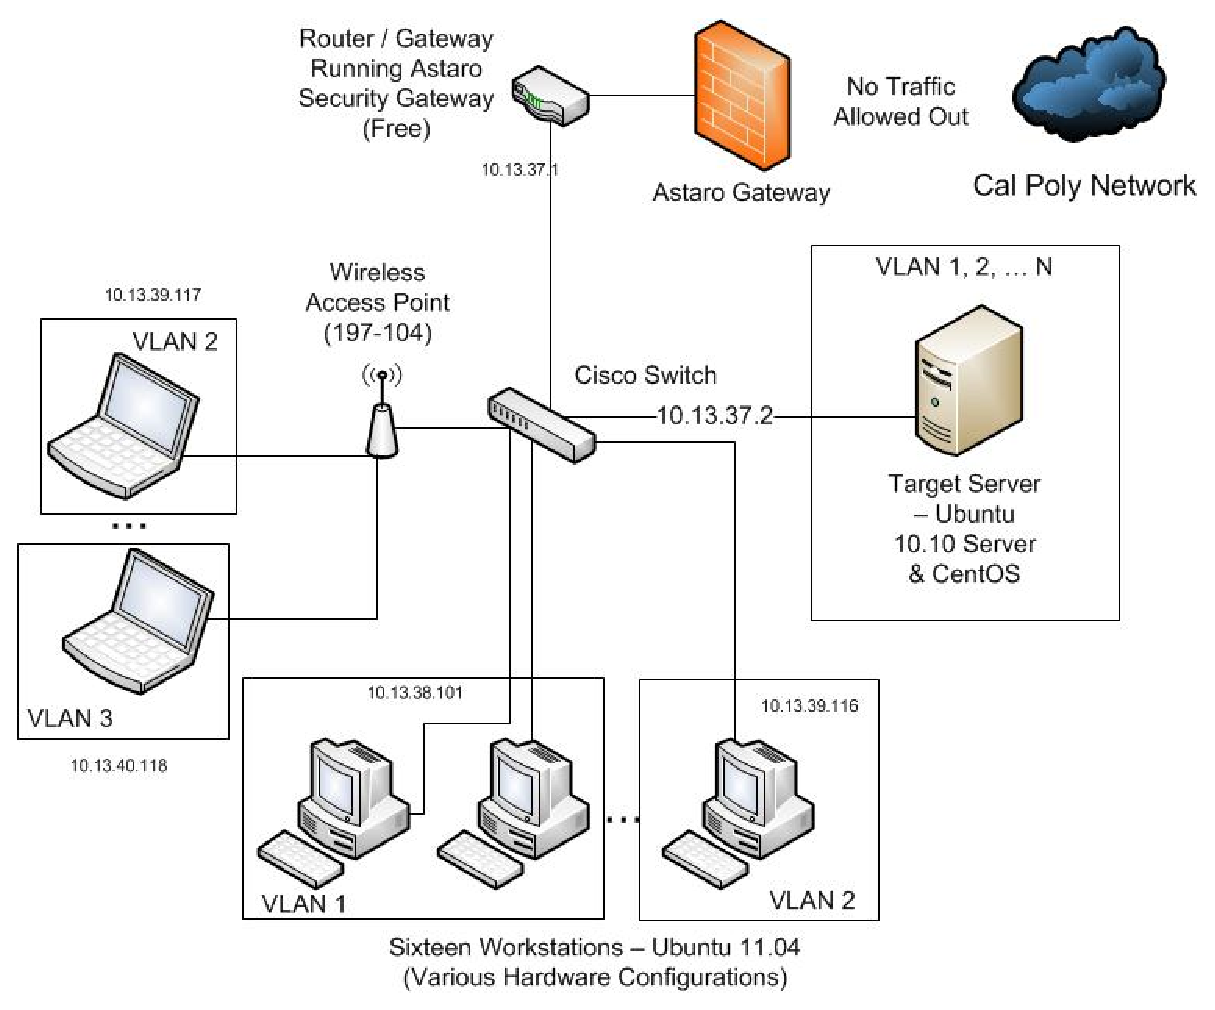
\includegraphics[scale=.50]{resources/dukenukem_network_diagram.eps}
\caption{A planned network diagram for the Duke Nukem CTF Scenario. Note: as
described in the problems and solutions sections, the planned network setup
did not end up including any of the described VLANs and the network connection
out of the lab was physically removed.}
\label{fig:dukeNetworkDiagram}
\end{figure}

\begin{figure}[here]
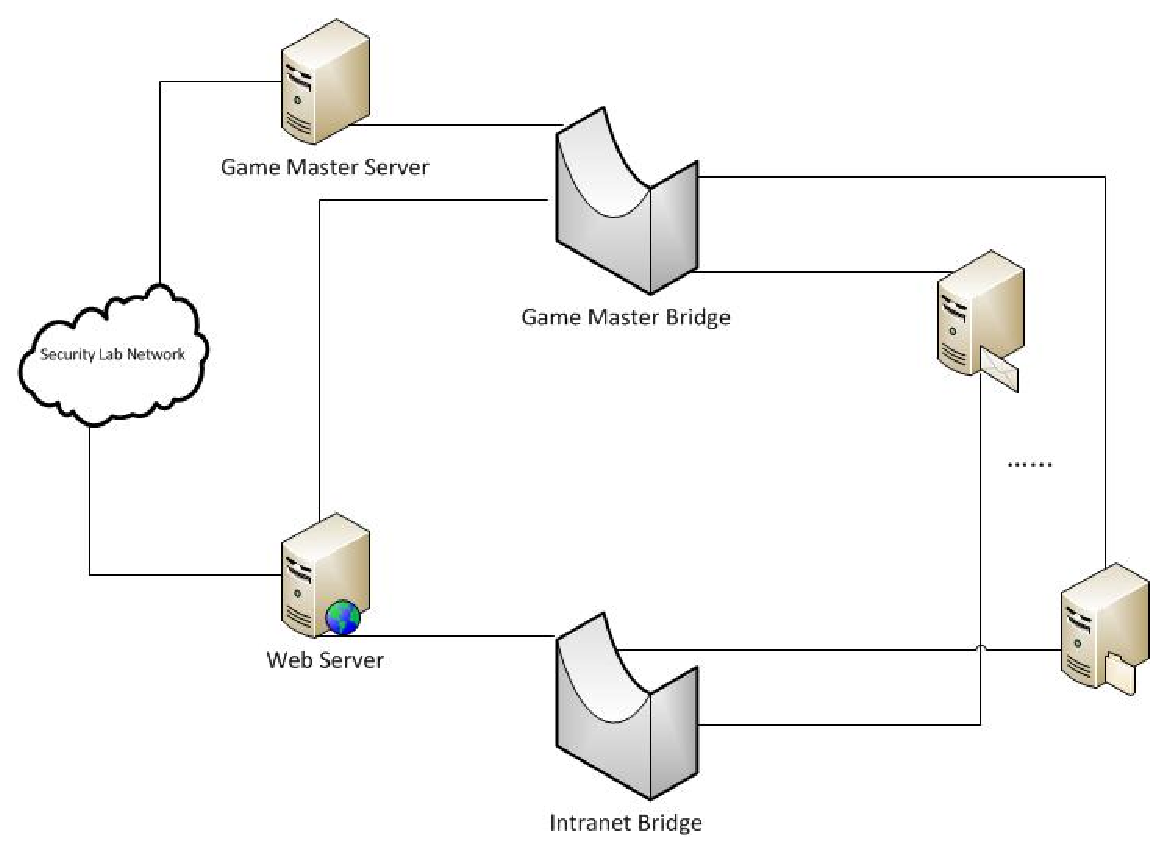
\includegraphics[scale=.75]{resources/dukenukem_intranet_diagram.eps}
\caption{A network diagram for the pseudo company's Intranet and Game Master
network.}
\label{fig:dukeNukemIntranetDiagram}
\end{figure}

\subsection{Game Day Results}
Competition began on May 22nd, 2011 at 10:00 a.m. with approximately 20 people
participating throughout the day. About a dozen people stayed for 10 hours until
7 p.m. when we called the game. 

Many of the participants had been regular attendees of our Security 101 sessions
and were able to find many of the flags directly related to the subjects we
covered. Groups were originally limited to at most three people, but as the
easier flags were all discovered participants began complaining about not
finding anything else. A few hinted that outside of the Security 101 sessions
they were very inexperienced and would like to join with the other groups
finding some of the harder flags to learn their techniques. After which, we
allowed the teams to grow to however large they liked.

There were two teams with experienced players and in each team someone with a
BackTrack Live CD. Since our servers were unpatched Ubuntu 10.10 installations,
they were able to use the automated tools supplied in BackTrack to exploit
known issues with Apache, MySQL, and PHP. These were not the intended attack
vectors. Even though they were able to get a root shell, they weren't able to do
much more. Eventually they realized they wouldn't be able to score any points
for their team and backed off. 

The competition was fraught with a number of issues at the beginning. We had not
restricted user access to some potentially destructive commands or sensitive
folders. For instance, an exploit which allowed participants to gain shell
access also allowed them to delete every file in the web directory or emptying
files by rewriting to them. In another instance, users were allowed to create
massive files in the \textit{tmp} directory. The virtual machine was limited to
15 Gigabytes of hard-drive space and eventually the \textit{tmp} folder grew so
large it prevented anyone else from downloading script they'd written to help
them find flags. Eventually, the entire virtual machine was unusable and needed
to be re-imaged.

By the end of the competition, only one team realized there were other servers
in the network (even though they were informed at the start of the competition)
and they were able to capture a few additional flags. When one of the more
experienced teams was informed they missed the other servers, they reported a
tool they used to find hidden content in images was reporting the strong
likelihood of a message on one of the web pages. They had spent considerable
time and resources attempting to extract the message and capture the flag. Upon
our further investigation, it was discovered the image they were working on was
not one of our seeded plants. Instead it was one of the stock images we used
from the original website we copied.

\subsection{Problems and Solutions}
\paragraph*{rm * -rf} As described in the \textbf{Game Day Results},
a few individuals were able to shut down the game by attacking the server
instead of finding the flags.

We were able to prevent the removal of files in the web directory by resetting
access to the files and directories. We still wanted them to be able to create
files to download their scripts, so we left one temporary folder open for them to
use. 

\paragraph*{Free Virtual Machine Servers} The server we were using to manage our
virtual machines was free and thus limited in the scale of available features.
Recall originally our plans called for a network setup such that the company's
Web server was on all VLANs in the network (see Figure
~\ref{fig:dukeNukemIntranetDiagram}). The limited feature set of our Virtual
Machine server did not include the ability to setup network cards for use with
VLANs. 

After two weeks of research and troubleshooting, we were not able to find a
suitable solution and instead did away with all of the VLAN requirements.
Additionally, we asked all participants to not attack each other's machines and
backup their data or use a Live CD if they were worried about breaking their
machines.

\paragraph*{BackTrack} One of our objectives was to test competitor's hacking
knowledge and abilities and not their ability to use pre-built scripts and
tools. Finding exploits in the services was not within the scope of this
competition. 

To prevent the use of tools which do all of the ``hacking'' for you, we decided
to change the design of the next CTF to the point they wouldn't be able to use
something like BackTrack by building our own services no one had ever worked
with before. 

\section{The Star Trek Scenario}
\label{stscenario}
\subsection{Objectives}
After the first CTF competition, we wanted to make our next focus to be on
solving two problems:
\begin{itemize}
	\item testing the individual's coding and hacking skills rather than their
	ability to find and use pre-built tools,
	\item and prevent the participants from breaking the servers (rather than the
	services) and ruining the game.
\end{itemize}

These would not only improve the overall game play and enjoyment, but would
help eliminate game down time spent repairing and restoring virtual machine
images. Additionally, by designing new services from the ground up we can
give participants experience with the common cause of vulnerabilities: poor
design.

Our first scenario was good for getting the uninitiated started in security,
however, it did lack defensive objectives. While the first scenario focused
mainly on attacking servers and their services, we needed to even the importance
of defending to better align the game with a real world scenario.

Lastly, players of the first competition noted in their feedback they wanted
more teamwork based cooperation. Specifically, those with little to no security
experience had a tough time working out the solutions and would have liked to
work with others outside of their team to strategize and learn techniques. The
standard method of team formation usually results in those who know each other
and have similar expertise tightly grouping together. This tends to vary
experience by groups rather than the individuals in the group and creates a
hording of knowledge in which the less experienced gain little from
participating. For this scenario, we wanted to move away from this particular
method.

\subsection{Design}
\label{stdesign}
To ensure no participant would be able to use pre-built tools to exploit
vulnerabilities, we chose to design services one might program during the first
implementations of a ship from Star Trek. This design was chosen
for two reasons: in the summer of 2011 Netflix began streaming every episode of
every Star Trek series \cite{Netflix}, and we couldn't find anyone who
had created such services or written anything to exploit such services. A
listing of these services and their designs can be found in \textbf{Game Play}
and \textbf{Services} sections ~\ref{stgameplay} and ~\ref{stservices}
respectively. Our new approach, described in the following sections, also
allowed us to make changes to the game play to focus more on team based play.

\subsubsection{Game Play}
\label{stgameplay}
The new game design was made to resemble a WarGame style of play consisting of
only two teams each with their own server to manage. We were even fortunate
enough to provide both teams with their own rooms to work in secrecy. Both
teams initially received identical copies of each service. Their goal to find
and patch vulnerabilities in their services then turn around and exploit the
same vulnerabilites in the other team. If a team could keep their services
responding and pass basic functionality tests they would score points. However,
if their services become unresponsive or failed the tests, whether their own
fault or the opposing team, they would stop receiving points while the opposing
team would score additional points.

We also wanted to give those participants with little or no hacking (or even
coding) experience something entertaining and contributory to do. Since these
services should be fully functional and collectively represent a star ship, then
it stands those who feel they can't ``hack" could fly the ship around and
score points for their team by shooting the other team's ship.

Team formation also changed. Now, no one knew which team they were playing on
until they showed up to the event. Each new person walking through the door was
automatically assigned to the oposing team assigned to the person before them.

\subsubsection{Score Keeping}
\label{stscorekeeping}
Since the game play was more complex than just doing tasks and getting scoring
for a flag. To have some form of live understanding the how the game is being
played to create a scoring metric to have a winner/score. Plus they had
admin access to their server and would have acess to source code and be compiling
their service.

We needed the score keeping to be more difficult to break than to play the game 
within the time frame of the game. To do this we needed to make the score keeper
as invisible as possible for the server and the score keeping partialy handled with
the base funcitonality given to the players to compile their service. [ see base 
functionality]. Also need to prevent the ability to spoof traffic.

\paragraph*{Scoring Schemes} Our metric for scores:
\begin{itemize}
  \item \textbf{Up-Time} - The main method for scoring points and
  represents the hacking side of the game. Scores are based on the accumulated
  time each service was responding to requests and passing the base-functionality tests. 
  \item \textbf{Communications} - Secondary encryption challenges.
  \item \textbf{Damage Dealt} - Teams may gain points not by hacking but by
  playing the game and fireing weapons as the opposing team's ship.
\end{itemize}

Both the communication and damange metics exist to add other challenges to
broden the interest for the game.

\paragraph*{Score Keeping}
Reasons for internal.
Since they can modify their code completely. We need some way on their side of
in check and making sure their service was keeping some form of base functionality.

External
Allows us to manage the scores and have other game play scoring aspects to the game.
This communicates witht he internal functionality checking.

%Implementations
Two main parts of the score keeping the base functionality within a service and
the VM / server designated to doing.

Base Functionality 
Check to state of the service.
If it passed it would report to the score keeper that that service is good.
If it failed it would report that the service did not meet base functionality would
be reported to the score keeper.
If the service was off then it would not be able to notify the remote server at all
that the service was up and the score keeper server would default tot the service
being off.

\subsubsection{Services}
\label{stservices}
On competition day, there were three implemented services in production for the
teams to fix with three additional services planned for release later in the
competition. (Each of the planned services and a brief description of their
functionality is listed at the end of this section).

Services are designed with two major parts: the built-in (or base)
functionality, and the competitor's implementation.

The base functionality was implemented by us and provided in unlinked
pre-compiled form for each team to build on top of. It is meant to represent the
initial implementation of a ship's services as made by first year ship
programmers. There are a few seeded vulnerabilities and even more hidden in poor
and hastily made designs. Base implementation of a service is only responsible
for:

\begin{itemize}
    \item providing only the most basic level of support and implementation
    necessary for the service to run, 
    \item setting up the network support required for running the service,
    \item listening on an assigned port, accept incoming connections, and pass
    on the connection to a handler which processes the incoming data,
    \item running base functionality tests on the competitor's implementation and
    pass on the results to the Score Keeper for scoring,
    \item and keeping a modest amount of internal book keeping specific to the
    service to ensure the honesty of a competitor's implementation.
\end{itemize}

While the exact functions for each service differ, every service's base
implementation has functions (defined as externals in header files)
for the competitor's code to call before finishing processing an incoming
request. For each of a service's base function, there is a corresponding
competitor's wrapper function to be called before the equivalent base function.
The location of the wrapper functions are stored in a structure as function
pointers defined in a shared header file between both implementations. These
wrapper functions allow the competitors the chance to perform their own book
keeping and sanitize inputs from requests before calling the base functions. A
diagram of the typical call stack and a snippet of the header files are
available in Figure ~\ref{fig:wraperStructEx}. This was one way for players to
patch vulnerabilities and design flaws.

To communicate between and control other services, each service had a
pre-defined packet structure mimicking an IP packet. Both teams started off with
the same structures but were allowed to extend the packets to fulfill any
future needs. The initial structure contained only enough fields to control each
specific command of a service. Any security or error checking features were left
up to the participants to develop and deploy. 

\begin{figure}[here]
\small
\begin{verbatim}
extern struct PowerFuncs {     

   void *(*request_handler) (void *confd);

      The following functions are your wrappers around the built-in / main 
      	 Power service functions. They will be used for testing your service 
         implementation and will not be called until your write your own
         implementation. At the end of each of your implementations, you must
         call the external equivalent functions. A diagram of the setup is
         bellow along with an example of the order of the function calls.

      Diagram:

      ----------------------------------------------------------
      |  request_handler                                       |
      |                                                        |
      |     ---------------------------------------------------|
      |     |  additional_function                             |
      |     |     (if you want to add additional               |
      |     |     checking or functionality to add security)   |
      |     |                                                  |
      |     |     ---------------------------------------------|
      |     |     |  wrapper_function                          |
      |     |     |     (for your book-keeping)                |
      |     |     |     EX) pow_funcs.wadd_power(int, int)     |
      |     |     |     ---------------------------------------|
      |     |     |     |  built-in_function                   |
      |     |     |     |     EX) add_power(int, int)          |
      |     |     |     |                                      |
      ----------------------------------------------------------

      Function Call Example:
         
      --> Incoming Connection Request
            |--> Connection Accepted
            |--> pow_funcs.request_handler(connection_file_descriptor)
               |--> additional_function(...)
                  |--> pow_funcs.wadd_power(int, int)
                     |--> add_power(int, int)
                  |--> send_packet(struct PowerHeader, socket_fd)

   int (*wregister_service) (int, int);
   int (*wunregister_service) (int);
   int (*wadd_power) (int, int);
} pow_funcs;
\end{verbatim}
\caption{A snippet of the provided header file for the Power service. It
describes the structure and use of the wrapper functions as well as
demonstrating the data flow of incoming requests.}
\label{fig:wraperStructEx}
\end{figure}

\paragraph*{Power} The critical service of each ship responsible for managing
and distributing a fixed amount of available ship power to all other running
services. A service may only run while it has been allocated power. Should a
service lose power, it shall be stopped and remain non-responsive until power is
restored. If the power service itself is shutdown or crashed, all other
services would be taken offline.

\paragraph*{Engines} Just like the engines in the star ships with support for
both impulse and warp speeds. The engine service is only concerned with
managing either engine's current power allocation and speed as well as ensuring
their health. Each engine leaks varying amounts of radiation which if not
dissipated could damage the engines to the point they are no longer functional.
Scotty can fix engine damage, but he's not a bloody miracle worker; he can only
work so fast!

\paragraph*{Navigation} Responsible for setting a ship's course, updating the
ship's internal representation of the map, and managing the engines.

\paragraph*{Communications} Independent of all other services except for the
power service, and instead of managing some aspect of a ship, presents each team
with a number of cryptography puzzles to be decrypted, solved, and posted back
to the Score Keeper for validation.

\paragraph*{Weapons} Shoots at a ``service''.  If the shooter is within range
and there are no shields protecting the targeted service the shooter receives
points for damaging their opponent.

\paragraph*{Shields} Temporarily protects a service from opposing weapons fire.

\subsection{Game Day Results}
The competition started around noon on November 5th, 2011 with four participants
and three of the services in production. Those services were the power, engines,
and navigation. The others had not yet been implemented, but were planned for
release some time at the end of the first day or during the start of the second
day of competition.

Over the next three or four hours both teams were still reading through the
documentation and asking questions trying to figure out the structure of the
game and the code. At least we thought they were reading the documentation.
Both teams would read a bit of the documentation and then start asking a
dozen or so questions each. Almost all of which could be answered if they
continued reading. It became quite irritating quite quickly especially as
the questions started to move towards exploiting the game rather than
playing it. Very little code was actually being written, but design flaws and
vulnerabilities were slowly being realized.

One or two members of Team A had previous experience in UNIX System
Administration and immediately began setting up monitoring tools to track
incoming requests and log the commands executed by each service. After which
they moved their focus to the operating system running their services and
attempted to ``secure'' it instead of their services. A few hours later and they
abandoned this approach. Eventually they settled on simply not processing any
incoming requests in their engine and navigation services. They effectively
produced a reverse denial of service.

Team B on the other hand, situated in the neighboring conference room decided to
start by developing tools to help them manage the services. (The initial
implementation provided no user friendly means to control a service. A member
would have to format a packet, open a connection to the service, send the
byte stream through the connection, and process any returned information.)
Through this management tool the team was able to track command requests between
services and drop unexpected incoming requests. Given the sequence of events for
each service's commands, the team could select the authentic commands and dump
any malicious ones. This was a great start for the team as they were able to
reap quick results.

Up until this point Team A had been setting up connections and sending ``random''
bytes of data to Team B's services. Since the original implementation was
faulty, these connections and incorrect data often crashed Team B's services,
causing them to fail tests and costing them points. When the new filter went
into place, these malicious attacks were almost completely eliminated.

Later on that night Team B started on their design for a basic level of
encryption. 

\subsection{Problems and Solutions}
\paragraph*{Lack of Experience Among Players} No one here really knows how to
exploit code, and those that do didn't participate.

For the first event we offered Security 101 sessions every Saturday leading up
to the competition to help prepare players and get them inspired. Because of
our lack of availability we weren't able to get a similar series setup. We
don't want to suggest correlation implies causation, but there was an obviously
lower attendance for the second competition.

\paragraph*{Stagnation} While one team outright dumped all incoming requests, 
the other did essentially the same thing by hardening access to their services
such that anyone not remotely logged-in into their server could not gain
control. Ultimately a good achievement, however, game play began to stagnate.

An easy fix would be to require all services to have an open public interface.
Instead of giving teams control of the server and the ability to lock others
out, anyone should be able to control a Team's services. This does bring up the
possibility of each team's ship experiencing erratic behavior (such as rapid
navigation changes and little to no movement across the game's map) but this
can be redefined as desired behavior. Such behavior can serve as motivation for
a team to work on ways to prevent the attacks or increase the attacks on
another team to bring their ship down first.

\paragraph*{Short On Time} One quarter to design, implement, and test completely
custom services and wrap them up into a game is not enough time for only two
people. You say you're going to work on it over the break, but good luck keeping
priorities.

At least two more people and one more quarter would help prevent slipping and
bad code (see next problem).

\paragraph*{Bad Tests} We started performing our implementation tests one and a
half weeks prior to the competition. While were able to catch and solve a few
big problems before the last minute, we weren't able to perform a ``dry-run'' of
game and iron out some other major issues between the Score Keeper and the
services. A fare and functional Score Keeper is key to a successful CTF
\cite{BlackHat2004}. Without the dry-run, we weren't able to find logic and
design flaws in our service tests and reporting which severely affected game
play.

Ideally, all code (services, Score Keeper, helpers, etc.) should begin
undergoing final implementation tests and debugging four weeks out from the
competition and integration tests done two full weeks out culminating in a
complete dry-run of the game. All services and Score Keeping should be fully
implemented and tested before integration testing begins. Additionally, at least
one virtual machine image should be created and saved for each of the following
(and will not be used for the competition):

\begin{itemize}
  \item a clean (without any game code) and fully configured server
  \item for each team, a working (with all game code included) instance which
  also contains and passes all implementation and integration tests
  \item for each team, the final working copy distributed at the start of
  competition
\end{itemize}

\paragraph*{Code Management} Each team's code had slightly different
configurations which had to be changed by hand within a single code base. With
10 to 12 changes to make in each service's code, insuring all changes were
properly made before each update was difficult under pressure. The design of
our Score Keeper (see Section ~\ref{stscorekeeping}) required all service
specific configurations to be contained within the pre-compiled source code
provided to each time. On a few occasions configuration settings for one team
made it into the compiled version of the other team. Resulting in services not
starting up, not communicating properly with other services, or communicating
incorrect results to the score keeper.

Ideally the services would have been written such that no updates were ever
needed to be pushed to servers during game play, however, other problems
inhibited this solution. 

Because of the way we decided to authenticate service status updates with
the proper team (as described in Section ~\ref{stscorekeeping}), we would
not be able to keep all configurations in a common header file. Instead we
should have either created two code bases (one for each team) with
configurations which don't change, or use a simple script to write all unique
configurations, compile the service, and push the update to the team's server.
The former would introduce the problem of ensuring both code bases were
synchronized with the proper updates. A simple solution, but one just as error
prone and no less irritating. The latter solution would take little time to
implement and cut update hassles down to a simple command line execution.

\paragraph*{Open-BSD} During the first competition, we had a
number of people trying to attack the server's services rather than finding the vulnerabilities
we created. Servers in the first competition were unpatched Ubuntu Server 10.10
instances with a number of open network services. Since this go around we didn't
need things like PHP, Apache, MySQL, etc., a stripped down operating system
capable of compiling code and running our network processes was ideal. After the
initial configuration, users would not have sudo-er privileges or be able to
install new packages. 

However, during our integration testing, we ran into a number of problems
getting the services to start up and behave properly. All code was POSIX
compliant but services had difficulties opening and binding sockets as well as
sending and receiving data. Limited remaining time (see \textbf{Short On Time}
and \textbf{Bad Tests}), we were not able to solve the problem and instead
switched to fully patched Ubuntu Server 11.10 instances with no sudo-er
privileges and without Apache, PHP, or MySQL installed. 

\section{Scenario Analysis}


\section{The Next Ideal Solution}
\subsection{Game Play}
Stick with the scenario [star trek] of large teams pitting against each other 
but create a bigger breadth of tasks and ways of winning similar to [scenario 1].
In addition create a visual front end to the game for the video game aspect.
By doing this you could create diversity in the game to help encourage newcomers
and retain them for longer.

\paragraph*{Visualization}
Adding visualization to services (e.g. navigation, weapons, and shields) would merge the game
between a hacking competition and video game similar to Hack Fortress \cite{HackFortress}.
We fill by adding this to the Star Trek Scenario ~\ref{stscenario} would not only
help encourage new players to get involved but help retain newcommers by having
an easier way to socially interact with thos who have more CTF experience.

\subsection{Network}

\subsubsection{VPN}
Create a VPN for the Sec Lab specifically for this event so people can participate any where
in the world. Make the event a multi school event. Similar to the [ucsb ctf]. This would
also allow students to practice when the security lab is closed. This also could be used
for the design of long term (e.g. Quarter Long) CTFs.

\subsection{Services}

\paragraph*{Adding Depth}
The custom services provided to players needs to have added functionality to add depth
to the service and making the service not as straight forward to secure.

\paragraph*{Denial of Service}
One of the vital issues with the services of Star Trek Scenario ~\ref{stscenario} is the
score keeping and over arching design was not able to prevent a teams denial of service
from other teams. This could be fixed by modifiying the score keeper to be integrated with
the a router \cite{BlackHat2004}, or wrapping all send and recv socket calls which
would be required to be used by the teams so that the data is sent to Score Keeper 
to make sure packets are being accepted and responded to accordingly for all teams.

\paragraph*{Library}
Create libraries to make it easier to create new services. Possibly make a generic base
functionality. This way it can be easier to create new services and so more time can
be spent on adding depth to the functionality of the service.

\paragraph*{Game Time Compile and Submit}
Add a way for players to automatically compile their code and the snapshot of that code
to the a repository. This would allow for a post game analysis of code. Possibly using
code Covarity [eric's paper] to see how robust the code is and compare it to scores
that team received.

\subsection{Score Keeper}

\subsubsection{Obfuscation}
The score keeper needs to be more sureptitious, internally (i.e. Base Functionality) and
externally (i.e. score keeping server).

\paragraph*{Internally}
To better deter players from reverse engineering our base functionality ncrypted packing of the base functionality, would be an extra deterant of people being
able to reverse engineer the base functionality.

\paragraph*{Communication}
We had encryption and some form of basic authentication by using a password.
Needs to be better.

\paragraph*{Externally}
Make your own virtual router to put your score keeper behind so that it makes it
more difficult to directly connect tot he score keeper but also allows you to in a central
point of score keeping see everything going on the network.
%ghetto hackerz did this

\subsubsection{Scoring Metrics}
If you can generate a flag capturing means of qualifying for points it is a bit easier
[scenario one - scoring] however if the game play is similar to [game 2] then there
needs to be a better metric than just checking the up times and down times of those machines.
They definitely could be a factor in the score but shouldn't really be the majority of the score.
create a means of hacking the server having some form of potentially layered affect on their
services so you can be more granulated or score and possibly modify points for scoring
offensively and defensively

\section{Other Suggestions And Things to Avoid}
For things specific to our and possible future CTFs at Cal Poly, the following
is a list of suggestions and things which should be avoided that may not have
been covered in a previous section or are important enough to be reiterated:
\begin{itemize}
    \item \textbf{Teaching} The competitions held in the immediate future should
    be expected to still have a large base of limited experience participants.
    Thus, the security workshop series should continue leading up to competition
    to cover topics which may appear in the scenario. It should not only help
    increase the number of participants, but also increase the level of play,
    enjoyment, and learning through the competition.
    \item \textbf{Advertise} Get competition details out every week (usually in
    conjunction with the 101 sessions). Be sure to get into the various
    department mailing lists (CSC, CPE, etc.). Posters should be up no later
    than two weeks prior to the competition.
    \item \textbf{No Experience Necessary?} We've tried using it in while
    advertising for both competitions, but no matter what, it didn't seem to
    help get the crowds we expected. There may be varying understandings of the
    phrase, but something along the same lines should stressed to those warry
    to participate.
    \item \textbf{Room Reservations} Reserve Bonderson rooms WELL in advance and
    confirm the reservation at least a month out. Don't forget to double check
    who has card swipe access.
    \item \textbf{Timing} Being on a quarter system presents a number of
    difficulties while selecting a date to host the competition. We found the end
    of week six might be the ideal time to avoid conflicts with midterms.
    However, use best fit (least number of conflicts) when picking a date
    knowing no weekend you chose is ever going to be perfect. Mind the holiday
    weekends, midterms, sporting events, or other club functions.
    \item \textbf{No all nighters}. It should go without saying. You're mainly
    going to be crashing and you'd rather be up all night during the
    competition rather than working on only a few hours of sleep and heading
    towards 56 hours without sleep.
    \item \textbf{Documentation} You're probably going to writing a report
    (maybe even one like this) and documenting before you begin work (ideally)
    or while you're working will greatly help in the future.
\end{itemize}

\section{Conclusion}

\newpage
\nocite{*}
\section{Bibliography}

\bibliographystyle{IEEEannot}

\bibliography{finalpaper}

\newpage

Work Distrobution

\end{document}
